% \documentclass[a4paper]{article}
\documentclass[12pt]{extarticle}
\usepackage[a4paper, left=1.5cm, right=1.5cm, top=1.5cm, bottom=2.0cm]{geometry}
\usepackage{graphicx} % Required for inserting images
\usepackage{caption}  % for continuedfloat

\usepackage{lscape} % For landscape pages
\usepackage{afterpage}
\usepackage{pdflscape} % To create landscape pages that show as landscape in PDF viewer
\usepackage{parskip} % Adds white space between paragraphs


\title{stroke\_lsoa\_prediction}
\author{Anna Laws}
\date{May!!! 2025}

\begin{document}

\maketitle

\section{Introduction}

Derive coefficients for the age-admissions prediction model.

\begin{itemize}
    \item Calculate coefficients without IMD bands from SSNAP data
    \item Initial optimisation
    \item Optimisation with simulated annealing
\end{itemize}


\section{SSNAP data}

Admissions data at MSOA level is from HES, 2017 to 2019 inclusive, and includes all stroke including some outside the usual stroke pathway that do not appear in SSNAP data.

HES data seems to only be valid for English MSOA so only use SSNAP data for English hospitals, assuming that patients based in Welsh MSOA only go to Welsh hospitals.

Take the subset of SSNAP data in England from 2017 to 2019 inclusive to match the HES data. Combine the age bands available and place patient data in the following age bands: under 65, 65--70, 70--75, 75--80, 80 and over. Divide the total number of strokes in each age band by three to find the annual stroke admissions. Scale up the annual admissions by the ratio of the total admissions in the HES and in the SSNAP data, around 1.45.

Take England population data from January 2019 and combine into the same five age bands. Table~\ref{tab:ssnap_coeffs}.


\begin{table}
\centering
    \caption{Stroke coefficients from SSNAP data. England population is 56.3 million in January 2019 and total annual strokes are 80958.}
    \begin{tabular}{crrr}
    Age Groups & Percentage of all population & Annual admissions & Probability of stroke given age \\
    \hline
    <65 & 81.6\% & 18737.7 & 0.04\% \\
    65--69 & 5.0\% & 7395.3 & 0.26\% \\
    70--74 & 5.0\% & 10379.6 & 0.37\% \\
    75--79 & 3.4\% & 11654.6 & 0.60\% \\
    80+ & 5.0\% & 32790.8 & 1.16\% \\
    \end{tabular}
    \label{tab:ssnap_coeffs}
\end{table}


\section{IMD bands}

Use 5 this time. 20\%, 40\%, 60\%, 80\%, 100\%.

\begin{figure}
    \centering
    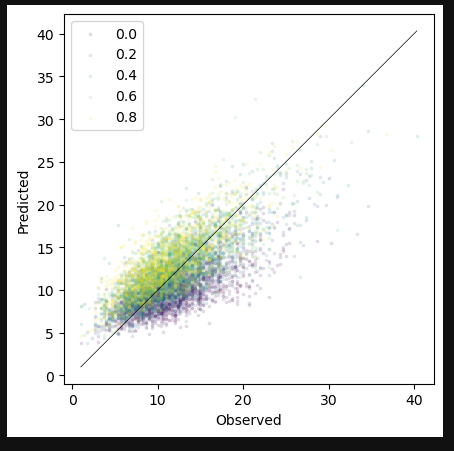
\includegraphics[width=0.5\linewidth]{images_imd_round2/admissions_ssnap_coeffs.png}
    \caption{Predicted vs observed admissions for the SSNAP-derived coefficients.}
    \label{fig:scatter_admissions_ssnap_coeffs}
\end{figure}

\section{Initial optimisation}

Start with the SSNAP-derived coefficients in Table~\ref{tab:ssnap_coeffs}.

Assume that different IMD quantiles will have different coefficients, and in particular that more-deprived quantiles will have higher coefficients (higher probability of stroke). 

Allow starting coefficients for each IMD band to be the SSNAP coefficients multiplied by a scaling factor in [0.6, 0.8, 1.0, 1.2, 1.4].
First calculate all combinations of these scale factors for the five IMD bands, then only keep combinations where the scale factor is larger in more-deprived quantiles.

For five quantiles in the order most deprived to least deprived, the final combinations are:
\begin{itemize}
    \item 0.6, 0.6, 0.6, 0.6, 0.6
    \item 0.8, 0.6, 0.6, 0.6, 0.6
    \item 0.8, 0.8, 0.6, 0.6, 0.6
    \item 0.8, 0.8, 0.8, 0.6, 0.6
    \item 0.8, 0.8, 0.8, 0.8, 0.6
    \item ...
    \item 1.4, 1.4, 1.4, 1.4, 0.6
    \item 1.4, 1.4, 1.4, 1.4, 0.8
    \item 1.4, 1.4, 1.4, 1.4, 1.0
    \item 1.4, 1.4, 1.4, 1.4, 1.2
    \item 1.4, 1.4, 1.4, 1.4, 1.4
\end{itemize}
There are 126 options in total.

We run the optimiser `scipy.optimize.minimize` with each set of starting coefficients in turn. The function optimises the values for all five age bands in all five IMD bands simultaneously, i.e. 25 coefficients are calculated with each pass. Coefficient values are restricted to between 0 and 1. The optimiser sets new values for the coefficients, calculates the admissions based on the area populations, and calculates the sum of squared residuals between predicted and observed admissions. A large penalty is applied for coefficients that do not increase with age band in each IMD band or that do not increase with deprivation in each age band.

The optimiser is not run on the MSOA-level data. First the MSOA are grouped into 10 (or 11 to use the full lot) MSOA and the admissions and populations summed for each group. This should reduce the effects of any randomness in the observed admissions data.
The admissions are predicted for these large groups and the sum of square residuals uses the difference between predicted and observed admissions in the group.

The separate MSOA-level data is used after the optimisation is finished to calculate an R-squared value for the fit. The resulting R-squared values for all admissions range from 0.59 to -0.81. 35 of the 126 options give an R-squared of at least 0.5. 

The coefficients of these 35 fits are usually different to one significant figure. 

Coefficients of best fit (left-to-right increasing age band, top-to-bottom decreasing deprivation):
\begin{itemize}
    \item 0.0006, 0.0035, 0.0043, 0.0070, 0.015
    \item 0.0005, 0.0032, 0.0043, 0.0067, 0.012
    \item 0.0004, 0.0028, 0.0038, 0.0062, 0.012
    \item 0.0003, 0.0027, 0.0035, 0.0057, 0.012
    \item 0.0003, 0.0021, 0.0034, 0.0046, 0.012
\end{itemize}

\subsection{Simulated annealing}

Use the 35 decent fits from the optimiser as inputs for another round of optimising with simulated annealing.
Round the coefficients to one significant figure (two for the over 80 band).
All 35 fits give a unique combination of rounded coefficients.

Run the annealing `scipy.optimize.basinhopping` with temperature 30 and step size 5e-5. So each coefficient can only jump up to 5e-5 in value, and a new set of coefficients with a result of 30 summed square residuals greater than the current best is likely to overtake the current best. Estimated residuals are around 240 for r-squared 0.59 down to around 265 for r-squared 0.50, so this temperature lets the new coefficients be a fair bit worse than best but not crazy worse.

Successfully ran for all 35 combos of input coefficients. Resulting r-squared values range from 0.587 to 0.598.
27 of these fits have r-squared that rounds to 0.60. 
These 27 fits have reasonably close coefficients?
So pick the best set and use the range of the 27 sets as a measure of confidence.

Best set r-squared values: 0.49678, 0.58430, 0.64385, 0.6147, 0.62772 for most to least deprived respectively and 0.59783 overall.

\begin{figure}
    \centering
    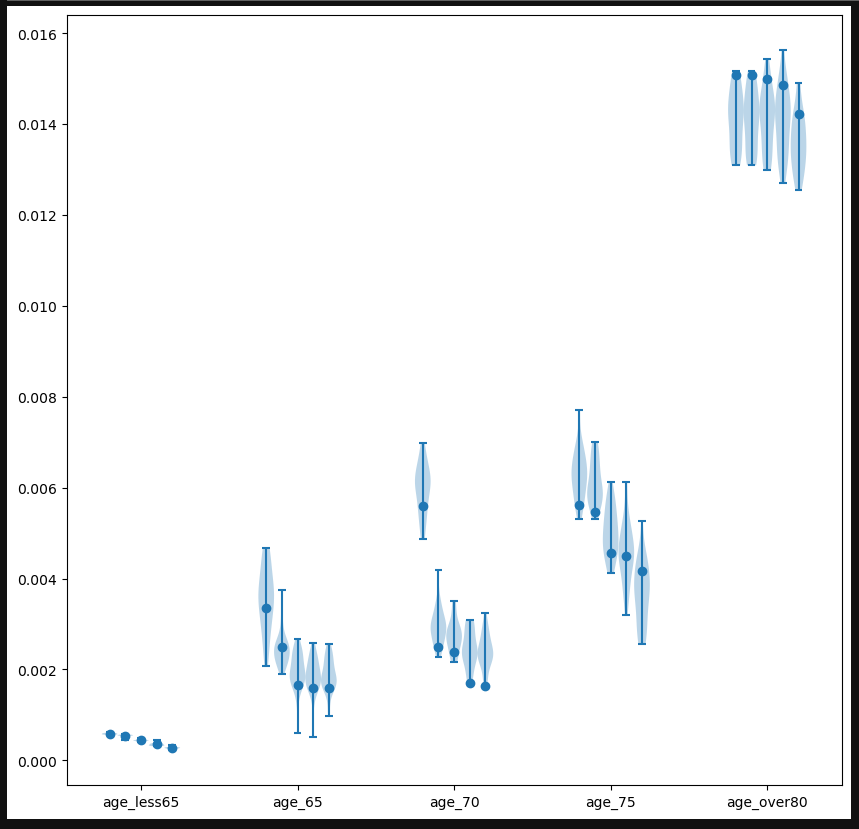
\includegraphics[width=1\linewidth]{images_imd_round2/best_annealing_coeffs_and_ranges.png}
    \caption{Best fit coefficients after annealing.}
    \label{fig:best_coeffs_and_range}
\end{figure}


\afterpage{%
    \clearpage% Flush earlier floats (otherwise order might not be correct)
    \thispagestyle{empty}% empty page style (?)
    \begin{landscape}% Landscape page
        \centering % Center table
\begin{table}
    \centering
    \begin{tabular}{rlllll}
        Depriv quantile min & <65 & 65--70 & 70--75 & 75--80 & Over 80 \\
        \hline
        0.0 & 0.00059 (0.00056--0.00061) & 0.0034 (0.0021--0.0047) & 0.0056 (0.0049--0.0070) & 0.0056 (0.0053--0.0077) & 0.0151 (0.0131--0.0152) \\
        0.2 & 0.00055 (0.00046--0.00058) & 0.0025 (0.0019--0.0037) & 0.0025 (0.0023--0.0042) & 0.0055 (0.0053--0.0070) & 0.0151 (0.0131--0.0152) \\ 
        0.4 & 0.00044 (0.00041--0.00048) & 0.0016 (0.0006--0.0027) & 0.0024 (0.0022--0.0035) & 0.0046 (0.0041--0.0061) & 0.0150 (0.0130--0.0154) \\ 
        0.6 & 0.00037 (0.00031--0.00044) & 0.0016 (0.0005--0.0026) & 0.0017 (0.0017--0.0031) & 0.0045 (0.0032--0.0061) & 0.0149 (0.0127--0.0156) \\
        0.8 & 0.00027 (0.00023--0.00033) & 0.0016 (0.0010--0.0026) & 0.0016 (0.0016--0.0032) & 0.0042 (0.0026--0.0053) & 0.0142 (0.0125--0.0149) \\
        \hline
        SSNAP & 0.00041 & 0.0026 & 0.0037 & 0.0060 & 0.0116 \\
    \end{tabular}
    \caption{Best coeffs after annealing}
    \label{tab:best_coeffs_annealing}
\end{table}
    \end{landscape}
    \clearpage% Flush page
}

\begin{figure}
    \centering
    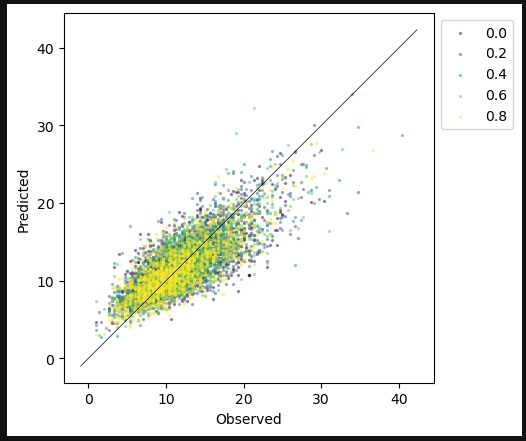
\includegraphics[width=0.5\linewidth]{images_imd_round2/admissions_predicted_vs_observed.png}
    \caption{Predicted admissions from best fit after annealing.}
    \label{fig:scatter_admissions_annealing}
\end{figure}

\end{document}
